% Shared style for all Git & GitHub lectures (same look as the N-body course)
\documentclass[11pt,a4paper]{article}
\usepackage[margin=2.3cm]{geometry}
\usepackage[T1]{fontenc}
\usepackage{lmodern}
\usepackage{upquote}   % straight quotes in monospaced text, so commands can be copied
\usepackage{microtype}
% keep '--' as two real hyphens in monospace text (commands like --version)
\DisableLigatures[-,<,>]{family=tt*}
\usepackage{booktabs,enumitem,graphicx,xcolor}
\usepackage{array}
\usepackage{needspace}
\usepackage{longtable}
\usepackage{float}
\usepackage{tikz}
\usetikzlibrary{arrows.meta,calc,positioning,decorations.pathreplacing,shapes.geometric,fit,backgrounds}
\usepackage[most]{tcolorbox}
\usepackage{listings}
\usepackage{fancyhdr}
\usepackage[colorlinks=true,linkcolor=blue!50!black,urlcolor=blue!50!black,citecolor=blue!50!black]{hyperref}

\setlength{\parindent}{0pt}
\setlength{\parskip}{0.6em}
\setlength{\abovecaptionskip}{4pt}
\usepackage[font=small,labelfont=bf]{caption}
\setlist{itemsep=0.2em,topsep=0.3em}

% ---------- colours ----------
\definecolor{cbg}{HTML}{F6F8FA}
\definecolor{ckw}{HTML}{0B5CAD}
\definecolor{ccm}{HTML}{6A737D}
\definecolor{cst}{HTML}{B5451B}
\definecolor{cpart}{HTML}{1F6FB2}
\definecolor{cheavy}{HTML}{C0392B}
\definecolor{cgreen}{HTML}{2E8B57}

% ---------- terminal listings ----------
% In a terminal session, lines starting with "$" are what YOU type.
% Everything else is what Git prints back.
\lstdefinestyle{term}{
  basicstyle=\ttfamily\small, backgroundcolor=\color{cbg},
  frame=single, rulecolor=\color{black!15}, showstringspaces=false,
  breaklines=true, columns=fullflexible, keepspaces=true,
  aboveskip=0.6em, belowskip=0.6em, xleftmargin=4pt, xrightmargin=4pt,
  literate={\$\ }{{\textcolor{cgreen}{\$\ }}}2,
  upquote=true
}
\lstset{style=term}
\newcommand{\code}[1]{\texttt{\small #1}}

% ---------- boxes ----------
\newtcolorbox{history}{colback=yellow!8,colframe=orange!60!black,
  title={History},fonttitle=\bfseries\small,left=4pt,right=4pt,top=2pt,bottom=2pt}
\newtcolorbox{quickfact}{colback=purple!4,colframe=purple!55!black,
  title={Quick fact},fonttitle=\bfseries\small,left=4pt,right=4pt,top=2pt,bottom=2pt}
\newtcolorbox{keyidea}{colback=blue!4,colframe=blue!50!black,
  title={Key idea},fonttitle=\bfseries\small,left=4pt,right=4pt,top=2pt,bottom=2pt}
\newtcolorbox{pitfall}{colback=red!4,colframe=red!55!black,
  title={Pitfall},fonttitle=\bfseries\small,left=4pt,right=4pt,top=2pt,bottom=2pt}
\newtcolorbox{tryit}{colback=teal!5,colframe=teal!55!black,
  title={Try it},fonttitle=\bfseries\small,left=4pt,right=4pt,top=2pt,bottom=2pt,breakable}
\newtcolorbox{homework}[1]{colback=green!4,colframe=green!40!black,
  title={Homework #1},fonttitle=\bfseries\small,left=4pt,right=4pt,top=2pt,bottom=2pt,
  breakable}
\newtcolorbox{goals}{colback=gray!6,colframe=gray!60!black,
  title={Learning goals},fonttitle=\bfseries\small,left=4pt,right=4pt,top=2pt,bottom=2pt}

% Solutions always start on a fresh page, behind a clear warning.
\newcommand{\solutionspage}{%
  \clearpage
  \begin{tcolorbox}[colback=red!6,colframe=red!60!black,halign=center]
    {\Large\bfseries Solutions}\\[0.3em]
    {\small Stop here if you have not tried the homework yet.\\
    Attempt every task first, run the checker, and only then read on.}
  \end{tcolorbox}
}

% ---------- Git diagram styles (TikZ) ----------
\tikzset{
  commit/.style={circle,draw=black!70,fill=blue!10,minimum size=7mm,inner sep=0pt,font=\scriptsize\ttfamily},
  newcommit/.style={commit,fill=orange!25,dashed},
  tag/.style={draw,rounded corners=2pt,font=\scriptsize\ttfamily,inner sep=2pt},
  branchtag/.style={tag,fill=green!15,draw=green!40!black},
  headtag/.style={tag,fill=yellow!30,draw=orange!70!black},
  remotetag/.style={tag,fill=purple!10,draw=purple!60!black},
  area/.style={draw,rounded corners,minimum height=11mm,minimum width=33mm,align=center,font=\small},
  cmdarrow/.style={->,thick,>=Stealth},
  link/.style={->,thick,>=Stealth,black!70},
}

% ---------- header ----------
\pagestyle{fancy}
\fancyhf{}
\renewcommand{\headrulewidth}{0.3pt}
\fancyfoot[C]{\thepage}
\newcommand{\lecturetitle}[3]{%
  \fancyhead[L]{\small\textit{Git \& GitHub from Zero}}
  \fancyhead[R]{\small Lecture #1}
  \begin{center}
    {\Large\bfseries Lecture #1}\\[0.4em]
    {\LARGE\bfseries #2}\\[0.4em]
    {\small #3}
  \end{center}
  \vspace{0.5em}
}

\tikzset{
  cbx/.style={draw,rounded corners,fill=blue!6,minimum width=1.9cm,minimum height=8mm,align=center,font=\scriptsize\ttfamily,inner sep=2pt}}
\emergencystretch=4em
\begin{document}
\lecturetitle{6}{Remotes and GitHub: Sharing Your Work}{\texttt{clone}, \texttt{push}, \texttt{fetch}, \texttt{pull}, SSH keys, and your first GitHub repository}

\begin{goals}
\begin{itemize}
  \item Explain what a \emph{remote} is and what \code{origin} and \code{origin/main} mean.
  \item Set up GitHub safely: account, private email address, and an SSH key.
  \item Put a local repository on GitHub, and copy a GitHub repository to your computer.
  \item Use \code{git push}, \code{git fetch} and \code{git pull}, and understand ``ahead'', ``behind'' and ``diverged''.
  \item Fix a rejected push.
\end{itemize}
\end{goals}

\section{Why a remote?}

So far everything lived on one computer. That is risky (a lost laptop loses the project) and lonely (nobody else can see or add to it). A \textbf{remote} is simply \emph{another copy of the repository, stored somewhere else}, usually on a server that several people can reach. \textbf{GitHub} is the most popular place to keep one.

Remember Lecture 0: Git is \emph{distributed}. Your computer holds a complete repository, GitHub holds another complete repository, and a friend's computer holds a third. They are equals in structure; they stay in step because people \emph{send} commits between them.

\begin{figure}[H]
\centering
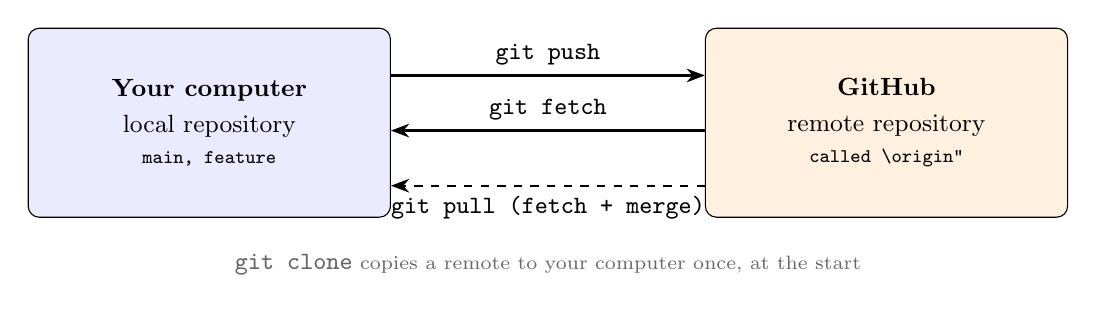
\begin{tikzpicture}[
  box/.style={draw,rounded corners,minimum width=4.6cm,minimum height=2.4cm,align=center,font=\small},
  arr/.style={->,thick,>=Stealth}]
  \node[box,fill=blue!8] (loc) at (0,0) {\textbf{Your computer}\\[2pt]local repository\\\scriptsize\ttfamily main, feature};
  \node[box,fill=orange!12] (rem) at (8.6,0) {\textbf{GitHub}\\[2pt]remote repository\\\scriptsize\ttfamily called \textquotedblleft origin\textquotedblright};
  \draw[arr] ([yshift=6mm]loc.east) -- node[above,font=\small\ttfamily] {git push} ([yshift=6mm]rem.west);
  \draw[arr] ([yshift=-1mm]rem.west) -- node[above,font=\small\ttfamily] {git fetch} ([yshift=-1mm]loc.east);
  \draw[arr,dashed] ([yshift=-8mm]rem.west) -- node[below,font=\small\ttfamily] {git pull (fetch + merge)} ([yshift=-8mm]loc.east);
  \node[font=\scriptsize,text=black!60] at (4.3,-1.8) {\code{git clone} copies a remote to your computer once, at the start};
\end{tikzpicture}
\caption{Two full copies of a repository. \code{push} sends your new commits up; \code{fetch} brings new commits down; \code{pull} is a fetch followed by a merge.}
\label{fig:remote}
\end{figure}

\section{Setting up GitHub}

Do these once. They take about ten minutes and are needed for the homework.

\subsection{Account and your private email address}

Create a free account at \url{https://github.com} and turn on two-factor authentication (Settings, ``Password and authentication''). Choose your user name carefully: it appears in every repository address.

In Lecture 1 you put your email address into \code{git config}, and in Lecture 5 you saw that every commit carries it. Commits pushed to GitHub show that address \emph{publicly}. GitHub offers a private ``no-reply'' address that works instead:

\begin{enumerate}
  \item In GitHub \textbf{Settings $\rightarrow$ Emails}, tick \emph{Keep my email addresses private} and, below it, \emph{Block command line pushes that expose my email}.
  \item The same page shows your no-reply address: a number, a plus sign, your user name, and \code{@users.noreply.github.com}.
  \item Tell Git to use it for future commits:
\end{enumerate}

\begin{lstlisting}
$ git config --global user.email "12345678+yourname@users.noreply.github.com"
\end{lstlisting}

Commits you have \emph{already} made keep the old address; the setting changes only new ones.

\subsection{Authentication: proving who you are}

To \code{push} you must prove that the repository is yours. GitHub no longer accepts your account password for this. There are two ways:

\begin{itemize}
  \item \textbf{HTTPS with a token.} Repository addresses start with \code{https://}, and you paste a long, secret \emph{personal access token} where a password would go.
  \item \textbf{SSH with a key} (recommended). Repository addresses look like \code{git@github.com:}\allowbreak\code{yourname/repo.git}. You create a pair of key files once and never type a password again.
\end{itemize}

An \textbf{SSH key} is a pair of files, like a padlock and its key. The \emph{public} half is the padlock: you may give it to anyone, and you put it on GitHub. The \emph{private} half is the key that opens it: it never leaves your computer.

\begin{figure}[H]
\centering
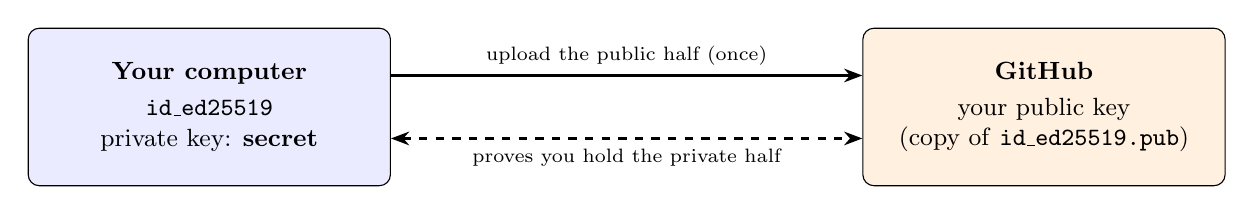
\begin{tikzpicture}[
  box/.style={draw,rounded corners,minimum width=4.6cm,minimum height=2.0cm,align=center,font=\small}]
  \node[box,fill=blue!8] (a) at (0,0) {\textbf{Your computer}\\[2pt]\code{id\_ed25519}\\private key: \textbf{secret}};
  \node[box,fill=orange!12] (b) at (10.6,0) {\textbf{GitHub}\\[2pt]your public key\\(copy of \code{id\_ed25519.pub})};
  \draw[->,thick,>=Stealth] ([yshift=4mm]a.east) -- node[above,font=\scriptsize] {upload the public half (once)} ([yshift=4mm]b.west);
  \draw[<->,thick,>=Stealth,dashed] ([yshift=-4mm]a.east) -- node[below,font=\scriptsize] {proves you hold the private half} ([yshift=-4mm]b.west);
\end{tikzpicture}
\caption{A key pair. Only the public half is ever uploaded.}
\label{fig:keys}
\end{figure}

\textbf{Create the key} (in a terminal; in Git Bash on Windows). Use your own email address as the label, and a passphrase when asked:

\begin{lstlisting}
$ ssh-keygen -t ed25519 -C "you@example.com"
Enter file in which to save the key (/Users/you/.ssh/id_ed25519):   <Enter>
Enter passphrase (empty for no passphrase):   <type one>
\end{lstlisting}

This creates two files in the hidden folder \code{\textasciitilde{}/.ssh/}: \code{id\_ed25519} (private) and \code{id\_ed25519.pub} (public). Print the public one and copy the whole line:

\begin{lstlisting}
$ cat ~/.ssh/id_ed25519.pub
ssh-ed25519 AAAAC3Nza...(long)... you@example.com
\end{lstlisting}

On GitHub open \textbf{Settings $\rightarrow$ SSH and GPG keys $\rightarrow$ New SSH key}, give it a title (for example ``my laptop''), paste the line, and save. Then test the connection:

\begin{lstlisting}
$ ssh -T git@github.com
Hi yourname! You've successfully authenticated, but GitHub does not provide shell access.
\end{lstlisting}

That message is success: GitHub knows you, and (as it says) does not give you a command line on its servers. The first time, SSH asks whether to trust the server; check the fingerprint against the one in GitHub's documentation, then answer \code{yes}.

\begin{pitfall}
Never share, e-mail or upload the file \emph{without} \code{.pub} (the private key), and never commit a \code{.ssh} folder. If you suspect it leaked, delete the key on GitHub and create a new pair. The passphrase protects the file if your laptop is stolen.
\end{pitfall}

\begin{quickfact}
If you prefer HTTPS: create a token under Settings $\rightarrow$ Developer settings $\rightarrow$ Personal access tokens, give it only the \emph{repo} permission, and paste it when Git asks for a password. Your operating system can remember it (the \emph{credential helper}). Everything else in this lecture is identical: only the address style differs.
\end{quickfact}

\section{Putting a local repository on GitHub}

You already have a local repository. To share it:

\begin{enumerate}
  \item On GitHub click \textbf{New repository}. Give it a name and choose public or private.
  \item \textbf{Do not} tick ``Add a README'', ``.gitignore'' or ``license''. Those would create a first commit on GitHub that your local history does not contain, and the two histories would not fit together. You want an \emph{empty} repository.
  \item GitHub now shows its quick-setup page with the repository's address. Copy the SSH address.
\end{enumerate}

\begin{pitfall}
That page offers two snippets, and the wrong one can do damage. The \emph{first} (``create a new repository on the command line'') starts with \code{echo "\# name" >> README.md} and \code{git init}. It is for a \emph{brand-new, empty folder}. Run inside an existing project, it appends a stray line to your README. You want the \emph{second} (``push an existing repository''), which has three lines. One of them, \code{git branch -M main}, \emph{renames the branch you are currently on} to \code{main}, so check with \code{git branch --show-current} that you are on the branch you mean.
\end{pitfall}

The three commands, run inside your existing repository:

\begin{lstlisting}
$ git remote add origin git@github.com:yourname/hello-github.git
$ git remote -v
origin  git@github.com:yourname/hello-github.git (fetch)
origin  git@github.com:yourname/hello-github.git (push)
$ git push -u origin main
To github.com:yourname/hello-github.git
 * [new branch]      main -> main
branch 'main' set up to track 'origin/main'.
\end{lstlisting}

(Real output also shows progress lines such as \code{Counting objects}, left out here.) Line by line:
\begin{itemize}
  \item \code{git remote add origin <address>} gives the remote a short name. \code{origin} is the conventional name for ``the place I got this from or share it with''; it is only a label.
  \item \code{git remote -v} lists your remotes. To change an address later: \code{git remote set-url origin <new-address>}.
  \item \code{git push -u origin main} sends the commits of the branch \code{main} to \code{origin}. The \code{-u} (``upstream'') makes your \code{main} \emph{remember} that it belongs with \code{origin/main}, so that afterwards a plain \code{git push} or \code{git pull} is enough.
\end{itemize}

\section{Copying a repository: \texttt{git clone}}

To get an existing repository, for example a friend's, you \emph{clone} it. On GitHub the green \textbf{Code} button shows the address.

\begin{lstlisting}
$ git clone git@github.com:friend/project.git
Cloning into 'project'...
$ cd project
$ git remote -v
origin  git@github.com:friend/project.git (fetch)
origin  git@github.com:friend/project.git (push)
$ git log --oneline --decorate
4c2511d (HEAD -> main, origin/main, origin/HEAD) Add notes
3db1fe7 Add README
\end{lstlisting}

One command created a new folder with the \emph{whole history}, set up the remote called \code{origin}, and checked out the main branch. (\code{git clone <address> mydir} picks another folder name.) You do not run \code{git init} first.

\section{Remote-tracking branches: \texttt{origin/main}}

Look at the log above: it shows both \code{main} and \code{origin/main}. They are different things.

\begin{itemize}
  \item \code{main} is \emph{your} branch. It moves when you commit.
  \item \code{origin/main} is a \textbf{remote-tracking branch}: your computer's \emph{memory} of where \code{main} was on \code{origin} the last time you talked to it. You never commit on it; Git moves it only when you push, fetch or pull.
\end{itemize}

Comparing the two tells Git (and you) whether you are ahead of, behind, or in step with the remote:

\begin{figure}[H]
\centering
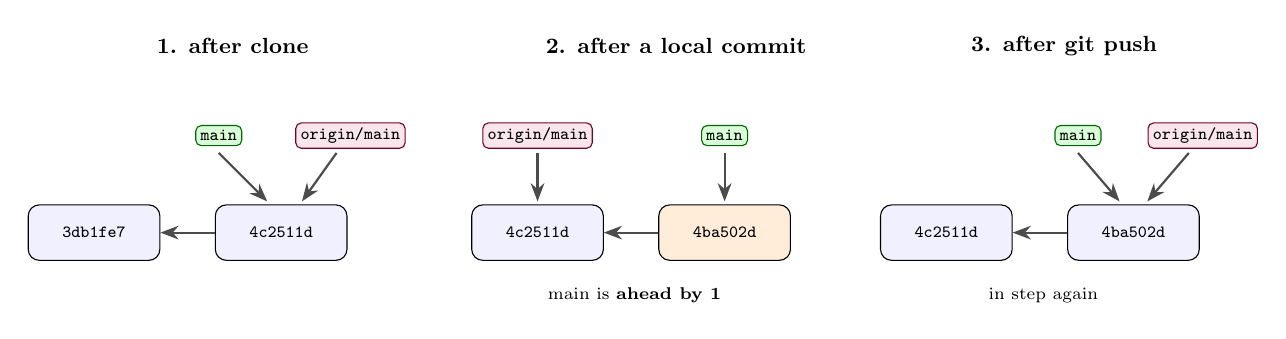
\begin{tikzpicture}[scale=0.88,transform shape]
  % panel 1
  \node[font=\small\bfseries] at (2.2,2.7) {1. after clone};
  \node[cbx] (a1) at (0.2,0) {3db1fe7}; \node[cbx] (b1) at (2.9,0) {4c2511d};
  \draw[link] (b1)--(a1);
  \node[branchtag] at (2.0,1.4) {main}; \node[remotetag] at (3.9,1.4) {origin/main};
  \draw[link] (2.0,1.15)--(2.7,0.45); \draw[link] (3.7,1.15)--(3.2,0.45);
  % panel 2
  \node[font=\small\bfseries] at (8.6,2.7) {2. after a local commit};
  \node[cbx] (b2) at (6.6,0) {4c2511d}; \node[cbx,fill=orange!15] (c2) at (9.3,0) {4ba502d};
  \draw[link] (c2)--(b2);
  \node[branchtag] at (9.3,1.4) {main}; \node[remotetag] at (6.6,1.4) {origin/main};
  \draw[link] (9.3,1.15)--(9.3,0.45); \draw[link] (6.6,1.15)--(6.6,0.45);
  \node[font=\scriptsize,align=center] at (8.0,-0.9) {main is \textbf{ahead by 1}};
  % panel 3
  \node[font=\small\bfseries] at (14.2,2.7) {3. after git push};
  \node[cbx] (b3) at (12.5,0) {4c2511d}; \node[cbx] (c3) at (15.2,0) {4ba502d};
  \draw[link] (c3)--(b3);
  \node[branchtag] at (14.4,1.4) {main}; \node[remotetag] at (16.2,1.4) {origin/main};
  \draw[link] (14.4,1.15)--(15.0,0.45); \draw[link] (16.0,1.15)--(15.4,0.45);
  \node[font=\scriptsize,align=center] at (13.9,-0.9) {in step again};
\end{tikzpicture}
\caption{\code{origin/main} (purple) stays where the remote was last seen. Committing moves only \code{main}; pushing moves both.}
\label{fig:tracking}
\end{figure}

\Needspace{9\baselineskip}
\code{git status} reports the comparison in words:

\begin{lstlisting}
$ git status
On branch main
Your branch is ahead of 'origin/main' by 1 commit.
  (use "git push" to publish your local commits)

nothing to commit, working tree clean
\end{lstlisting}

\begin{keyidea}
\code{origin/main} is only as fresh as your last contact. \code{git status} never phones GitHub: if a friend has pushed since, it will still say ``up to date'' until you \code{fetch}.
\end{keyidea}

\section{Getting others' work: \texttt{fetch} and \texttt{pull}}

A friend pushes a commit. Your computer does not know yet. \code{git fetch} downloads new commits and moves \code{origin/main}, but \emph{touches neither your branch nor your files}, so it is always safe:

\begin{lstlisting}
$ git fetch
From github.com:friend/project
   4c2511d..322927b  main       -> origin/main
$ git status
On branch main
Your branch is behind 'origin/main' by 1 commit, and can be fast-forwarded.
  (use "git pull" to update your local branch)

nothing to commit, working tree clean
$ git log --oneline main..origin/main        # what is new on the remote?
322927b Friend update
\end{lstlisting}

``Behind, and can be fast-forwarded'' is the easy case from Lecture 5: your branch just has to catch up. \code{git pull} does exactly a fetch followed by a merge, here a fast-forward:

\begin{lstlisting}
$ git pull
Updating 4c2511d..322927b
Fast-forward
 friend.txt | 1 +
 1 file changed, 1 insertion(+)
 create mode 100644 friend.txt
\end{lstlisting}

\subsection{When both sides have new commits}

The harder case: while you made a commit locally, your friend pushed one. Now the two copies have \emph{diverged}, exactly like the two branches of Lecture 5. Git protects the shared copy and rejects your push:

\begin{lstlisting}
$ git push
To github.com:friend/project.git
 ! [rejected]        main -> main (fetch first)
error: failed to push some refs to 'github.com:friend/project.git'
hint: Updates were rejected because the remote contains work that you do
hint: not have locally. This is usually caused by another repository pushing
hint: to the same ref. You may want to first integrate the remote changes
hint: (e.g., 'git pull ...') before pushing again.
\end{lstlisting}

\begin{figure}[H]
\centering
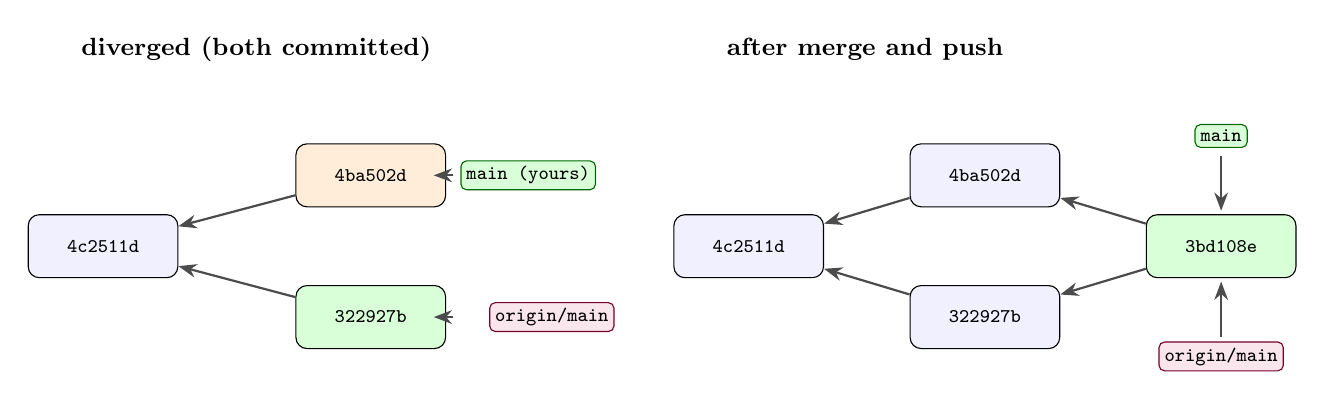
\begin{tikzpicture}
  \node[font=\small\bfseries,anchor=west] at (-0.4,2.5) {diverged (both committed)};
  \node[cbx] (a) at (0,0) {4c2511d};
  \node[cbx,fill=orange!15] (m) at (3.4,0.9) {4ba502d};
  \node[cbx,fill=green!15] (f) at (3.4,-0.9) {322927b};
  \draw[link] (m)--(a); \draw[link] (f)--(a);
  \node[branchtag] at (5.4,0.9) {main (yours)}; \draw[link] (4.45,0.9)--(4.2,0.9);
  \node[remotetag] at (5.7,-0.9) {origin/main}; \draw[link] (4.45,-0.9)--(4.2,-0.9);
  \node[font=\small\bfseries,anchor=west] at (7.8,2.5) {after merge and push};
  \node[cbx] (a2) at (8.2,0) {4c2511d};
  \node[cbx] (m2) at (11.2,0.9) {4ba502d};
  \node[cbx] (f2) at (11.2,-0.9) {322927b};
  \node[cbx,fill=green!15] (x2) at (14.2,0) {3bd108e};
  \draw[link] (m2)--(a2); \draw[link] (f2)--(a2); \draw[link] (x2)--(m2); \draw[link] (x2)--(f2);
  \node[branchtag] at (14.2,1.4) {main}; \draw[link] (14.2,1.15)--(14.2,0.45);
  \node[remotetag] at (14.2,-1.4) {origin/main}; \draw[link] (14.2,-1.15)--(14.2,-0.45);
\end{tikzpicture}
\caption{Left: your \code{main} and \code{origin/main} point at different commits. Right: a merge commit joins them; after the push both labels sit on it.}
\label{fig:diverged}
\end{figure}

The cure is the merge you learned in Lecture 5: first bring your friend's commit in, then push. Newer Git versions, however, insist that you \emph{choose} how \code{pull} should combine the two:

\begin{lstlisting}
$ git pull
From github.com:friend/project
   4c2511d..322927b  main       -> origin/main
hint: You have divergent branches and need to specify how to reconcile them.
hint: You can do so by running one of the following commands sometime before
hint: your next pull:
hint:   git config pull.rebase false  # merge
hint:   git config pull.rebase true   # rebase
hint:   git config pull.ff only       # fast-forward only
fatal: Need to specify how to reconcile divergent branches.
\end{lstlisting}

(Some of the hint lines are left out.) Notice that the fetch part already worked: \code{origin/main} moved. Only the combining step is waiting for your decision. We choose \textbf{merge}, which you know, and say so once for all repositories (rebase is Lecture 8):

\begin{lstlisting}
$ git config --global pull.rebase false
$ git pull --no-edit              # fetch + merge origin/main
Merge made by the 'ort' strategy.
 friend.txt | 1 +
 1 file changed, 1 insertion(+)
 create mode 100644 friend.txt
$ git push
To github.com:friend/project.git
   322927b..3bd108e  main -> main
\end{lstlisting}

The same thing, step by step, is \code{git fetch} followed by \code{git merge origin/main}. If the merge ever conflicts, resolve it exactly as in Lecture 5, then commit and push.

\begin{quickfact}
Never use \code{git push --force} to get around a rejection. It overwrites the remote with your version and \emph{deletes your friend's commits} from it. Beginners should treat it as forbidden until Lecture 8.
\end{quickfact}

\section{Branches and the remote}

A new branch exists only on your computer until you push it. Use \code{-u} the first time:

\begin{lstlisting}
$ git switch -c feature
$ git push -u origin feature
 * [new branch]      feature -> feature
branch 'feature' set up to track 'origin/feature'.
$ git branch -vv
* feature d74b2c7 [origin/feature] Add feature file
  main    3bd108e [origin/main] Merge remote-tracking branch 'origin/main'
$ git branch -r
  origin/HEAD -> origin/main
  origin/feature
  origin/main
\end{lstlisting}

\code{git branch -vv} shows which remote branch each local branch tracks; \code{git branch -r} lists the remote-tracking branches. To delete a branch on the remote once it is merged: \code{git push origin --delete feature}. (Your own \code{origin/feature} label disappears at the next \code{git fetch --prune}.)

\section{What GitHub adds}

The website shows your repository: files, the commit list, branches, and the \code{README.md} rendered as a front page. A README is written in \textbf{Markdown}, a plain-text format where \code{\# Title} is a heading, \code{**bold**} is \textbf{bold}, \code{- item} starts a list, and backticks make \code{code}. You can also edit a file in the browser (the pencil icon) and ``commit changes'' there. That creates a \emph{commit on GitHub}, which your local copy does not have until you \code{git pull}.

\begin{pitfall}
Everything you push is as visible as the repository: anyone can read a \emph{public} repository, and history keeps every old version. Never push passwords, keys or tokens (Lecture 2), even in a file you later delete.
\end{pitfall}

\Needspace{12\baselineskip}
\section{Homework 6}

\begin{homework}{6: Sharing}
\textbf{Part A: practice with a ``server'' folder} (no internet needed). The setup script creates \code{practice/hw6\_server.git}, a shared repository that plays the role of GitHub. From the course folder run:
\begin{lstlisting}
$ bash codeHints/L06/setup_hw6.sh
$ cd practice
\end{lstlisting}
Do the tasks in this order. To start over: \code{setup\_hw6.sh --reset} from the course folder.

\begin{description}[leftmargin=1.2em,style=nextline]
\item[6.1 Clone] Clone the server into a folder called \code{hw6} (\code{git clone hw6\_server.git hw6}) and go into it.
\item[6.2 Look around] Run \code{git remote -v}, \code{git branch -a} and \code{git log --oneline --decorate}. In \code{practice/hw6\_answers.txt} (next to the \code{hw6} folder; create it with \code{printf} or \code{echo}) write the line \code{remote=<the name of the remote>}.
\item[6.3 Commit locally] Create \code{mine.txt} containing \code{my work} and commit it as \code{Add my work}. \emph{Do not push yet.} Run \code{git status} and add the line \code{ahead=<number of commits ahead>} to the answers file.
\item[6.4 Your friend pushes] From the \emph{course folder} run \code{bash codeHints/L06/friend.sh}. Back in \code{hw6}, try \code{git push} and read the rejection. Set \code{git config pull.rebase false}, then run \code{git pull --no-edit}. Check \code{git log --oneline --graph}: there is now one merge commit.
\item[6.5 Push] Run \code{git push}. Your \code{main} and the server's \code{main} must now be identical.
\item[6.6 A branch] Create the branch \code{feature}, add a file \code{feature.txt}, commit it as \code{Add feature file}, and push it with \code{git push -u origin feature}.
\item[6.7 Question] Add the line \code{no-merge=<command>}: the one Git command from this lecture that downloads new commits \emph{without} changing your branch or your files.
\end{description}

\textbf{Part B: the real thing (optional, but this is why you came).} You need your GitHub account and the SSH key from this lecture.
\begin{description}[leftmargin=1.2em,style=nextline]
\item[6.8 Create and push] On GitHub create a new \emph{empty} repository called \code{hello-github} (no README). In \code{practice/} create the folder \code{hw6\_github}, run \code{git init -b main} in it, add a \code{README.md} with a heading line, commit, add the SSH address as \code{origin}, and \code{git push -u origin main}.
\item[6.9 Edit on GitHub, then pull] In the browser, edit \code{README.md} and commit the change on GitHub. Then run \code{git pull} locally and check \code{git log} shows the new commit.
\item[6.10 Look and check] Open the repository page on github.com and find your commits. Then run the checker.
\end{description}

\textbf{Check yourself:} from the course folder run \code{bash codeHints/L06/check\_hw6.sh}. Part A needs no network. Part B is checked only if \code{practice/hw6\_github} exists; if GitHub cannot be reached, that one check is skipped. All \code{PASS}, then compare with the solutions at the end of this lecture (or in \code{solutions/L06/}).
\end{homework}

\section{Summary}

\begin{itemize}
  \item A remote is another full copy of the repository; \code{origin} is the usual name for the one you share with. \code{origin/main} is your memory of where \code{main} was on it.
  \item Set up GitHub with a private no-reply email and an SSH key (public half uploaded, private half secret).
  \item \code{git remote add}, \code{git push -u origin main} publish a local repo (create it \emph{empty} on GitHub); \code{git clone} copies one.
  \item \code{fetch} downloads safely; \code{pull} is fetch plus merge. If both sides have new commits, pull (merge) first, then push. Never force-push.
\end{itemize}

\textbf{Further reading:} \emph{Pro Git}, Chapters 2.5 and 3.5; GitHub Docs, ``Connecting to GitHub with SSH''.

\solutionspage

\section*{Solutions to Homework 6}

\textbf{Part A.}

\begin{lstlisting}
$ bash codeHints/L06/setup_hw6.sh
$ cd practice
$ git clone hw6_server.git hw6
$ cd hw6
$ git remote -v                      # origin ... (fetch), origin ... (push)
$ git branch -a
* main
  remotes/origin/HEAD -> origin/main
  remotes/origin/main
$ echo "my work" > mine.txt
$ git add mine.txt
$ git commit -m "Add my work"
$ git status                         # "ahead of 'origin/main' by 1 commit"
$ printf 'remote=origin\nahead=1\nno-merge=fetch\n' > ../hw6_answers.txt
$ cd ../..                           # back to the course folder
$ bash codeHints/L06/friend.sh
$ cd practice/hw6
$ git push                           # rejected (fetch first)
$ git config pull.rebase false
$ git pull --no-edit                 # fetch + merge: one merge commit
$ git log --oneline --graph
$ git push
$ git switch -c feature
$ echo "feature" > feature.txt
$ git add feature.txt
$ git commit -m "Add feature file"
$ git push -u origin feature
\end{lstlisting}

\textbf{6.1--6.2.} \code{git clone} created \code{hw6} with the full history and a remote named \code{origin} that points at the server folder. The remote's name is \code{origin} (Git chooses it for a clone), hence \code{remote=origin}.

\textbf{6.3.} Your branch has one commit that \code{origin/main} lacks, so \code{git status} says ``ahead by 1 commit'' and \code{ahead=1}. Nothing is on the server yet.

\textbf{6.4.} The friend's commit reached the server after you cloned, so the two copies diverged and \code{git push} is rejected with ``fetch first''. Plain \code{git pull} on a recent Git stops with ``Need to specify how to reconcile divergent branches'' (after already fetching); \code{git config pull.rebase false} chooses merge. The merge commit is the \emph{one} merge commit the checker expects. (\code{git fetch} followed by \code{git merge origin/main} gives the same result.)

\textbf{6.5.} After the merge your \code{main} is ahead of \code{origin/main}, and a push is now a fast-forward for the server, so it is accepted.

\textbf{6.6.} \code{-u} records that local \code{feature} tracks \code{origin/feature} (the checker reads \code{branch.feature.remote} and \code{branch.feature.merge} from your repository).

\textbf{6.7.} \code{fetch}: it downloads and moves \code{origin/main} but changes neither your branches nor your files. \code{git pull} also merges.

\textbf{Part B.}

\begin{lstlisting}
$ cd practice
$ mkdir hw6_github
$ cd hw6_github
$ git init -b main
$ echo "# Hello GitHub" > README.md
$ git add README.md
$ git commit -m "Add README"
$ git remote add origin git@github.com:YOURNAME/hello-github.git
$ git push -u origin main
        (now edit README.md on github.com, "Commit changes")
$ git pull
$ git log --oneline                  # two commits
\end{lstlisting}

Replace \code{YOURNAME} by your GitHub user name. After the browser edit, GitHub is one commit ahead of you, so \code{git pull} brings it in as a fast-forward and your local \code{main} again equals GitHub's.

\Needspace{8\baselineskip}
\textbf{Common mistakes and fixes.}
\begin{itemize}
  \item Running \code{friend.sh} before cloning, or pushing before 6.4. Then there is no divergence and no merge commit, so the check ``exactly one merge commit'' fails. Run \code{setup\_hw6.sh --reset} and follow the order.
  \item \code{Permission denied (publickey)} when pushing to GitHub: the key is not added to your account, or the remote uses the wrong address style. Test with \code{ssh -T git@github.com}; check \code{git remote -v}.
  \item Creating the GitHub repository \emph{with} a README, then pushing: rejected, because GitHub has a commit you lack. Either create it empty (best) or run \code{git pull origin main --allow-unrelated-histories}, resolve any conflict, and push.
  \item Using \code{git push --force} to ``fix'' a rejection: not allowed here, it erases others' work.
\end{itemize}


\end{document}
